\section{GWAS of left ventricular trabeculation}
\label{section:GWAS_FD}
Early in mammalian heart development, the myocardium is composed of a loose network of fibers and sinusoids that forms sheet-like protrusions into the cardiac lumen. These structures in the inner layer of the myocard will give rise to the trabecular myocardium. In subsequent stages of heart development, the sinusoids disappear and the trabecular myocardium becomes more compacted towards the outer wall of the myocard, forming a thick, compact ventricular wall \citep{Chen2009,Yousef2009}. Failure of the myocardial compaction process leads to persistence of ventricular hypertrabeculation or non-compaction (NC). The majority of NC phenotypes are observed in the left ventricle (LV) \citep{Zambrano2002}. It remains unknown whether LVNC is a distinct disease or a shared characteristic of different cardiomyopahties \citep{Captur2013}. In addition to NC as a clinical phenotype, variation in trabeculation pattern and strength have also been observed in healthy volunteers from different ethnic backgrounds \citep{Kawel2012,Captur2015}. In this study, we aimed to map genetic variation to LV trabeculation phenotypes. Trabeculation is quantified via fractal analysis, which meassures complex patterns. The phenotype obtained is fractal dimension (FD), a unit-mess measure, that serves as a proxy for the complexity i.e. the level of trabeculation of the endocardial wall. The higher the FD measure, the higher the complexity  of the structure. Genotype to phenotype mapping was achieved by fitting a multi-variate LMM to FD meassurements derived throughout the heart.

\subsection{Data}
\subsubsection{Genotypes}
\label{sssec:gentoypes}

\paragraph{Quality Control.}Genotyping was carried out at the Genotyping and Microarray facility at the Wellcome Trust Sanger Institute, UK and Duke-NUS Medical School, Singapore. Genotypes were assessed in five batches using Illumina HumanOmniExpress- 12v1-1 (Sanger, two batches), Illumina HumanOmniExpress- 24v1-0 (Duke-NUS, two batches) and Illumina HumanOmniExpress- 24v1-1 chips (Duke-NUS). Probes targeting the same SNP on the different chip versions were confirmed to have the same sequence. SNPs were called via the GenCall software for clustering, calling and scoring of genotypes \citep{Teo2007}. For batches run on the same platform, genotype signals were combined and called in a single analysis, leading to three independent genotype batches: sanger12 (1,344 samples), Duke-NUS12 (284 samples), Duke-NUS3 (96 samples). Genotyping quality control (QC), phasing and imputation were conducted on a per-batch level. 

Prior to QC, rsID descriptions (chromosome, chromosomal positions and allele order) of the three batches were matched to the reference set used for imputation (combined UK10K \citep{UK10KConsortium2014} and 1000 Genomes \citep{Abecasis2012} reference panel) and ensembl human variation annotation (GRCh37p13, 15.04.2016) for rsIDs not included in the reference panel. rsIDs that matched to neither reference were removed from further analyses. The quality of the genotypes was evaluated both on a per-individual and per-marker level following an adapted quality control protocol of Anderson and colleagues \citep{Anderson2010}. Unless stated otherwise, the PLINK software (version 1.9) \citep{Purcell2007, Chang2015} was used for all QC analyses. In summary, the per-individual QC included the identification of individuals with discordant sex information, missing SNP rates (more than 3\% of SNPs not called) and outlying heterozygosity rates (outside 3 standard deviations of mean heterozygosity rate). Population substructures arising due to different ethnical origins of samples were examined by comparison of sample genotypes to genotypes of the HapMap Phase III study \citep{HapMap2005} from four ethnic populations. Samples that clustered with HapMap III individuals of caucasian ancestry were kept for further analyses. The per-marker QC included filtering of SNPs with missing call rate in more than 1\% of the samples and SNPs which significantly deviate from Hardy-Weinberg equilibrium (HWE, \(p < 0.001\)).  Table~\ref{tab:genoOverview} shows an overview of sample and SNP numbers before and after the QC described above. 
\\
% Table generated by Excel2LaTeX from sheet 'GenotypesSummaryHVOL'
\begin{table}[htbp]
  \centering
  \caption{\textbf{Overview of genotype data before and after quality control.}}
    \begin{tabular}{llrllrr}
    		\toprule
          & \multicolumn{2}{c}{\textbf{pre-QC}} &  &\multicolumn{3}{c}{\textbf{post-QC}} \\
          \cmidrule{2-3}\cmidrule{5-7}
          & samples (m/f) & \multicolumn{1}{l}{SNPs} & & samples (m/f) & \multicolumn{1}{l}{SNPs} & \multicolumn{1}{l}{genotyping rate} \\
            \cmidrule{2-7}
    \textbf{Sanger12} & 1344  (614/  730) & 719,665 & & 998 (463/535) & 677,036 & 0.997678 \\
    \textbf{Duke\_NUS12} & 284 (118/ 166) & 716,503 &  &179 (68/ 111) & 682,016 & 0.998253 \\
    \textbf{Duke-NUS3} & 96 (48/ 48) & 713,014 &  &62 (34/ 28) & 657,497 & 0.997916 \\
    \bottomrule
    \end{tabular}%
  \label{tab:genoOverview}%
\end{table}%

\paragraph{Phasing and imputation.} Phasing and imputation were conducted in two separate steps. The SHAPEIT software (version 2) \citep{Delaneau2012,Delaneau2013} was used to generate a set of estimated haplotypes based on the combined 1000 Genomes \citep{Abecasis2012} and UK10K \citep{UK10KConsortium2014} reference panel as genetic map. The same reference panel was used for the imputation of the samples’ genome-wide SNP genotypes via the IMPUTE2 software (version 2.3.0) \citep{Marchini2007, Howie2009}. 
\paragraph{Combining dataset.} The three genotype batches were combined after imputation and filtered again on a per-marker and per-sample level. SNPs with a certainty score of less than 0.4 in at least one of the batches were excluded from further analyses. None of the 631,877 common SNPs had to be removed due to significant differential missingness (\(p < 1e-5\)) across the three batches. After combining the three datasets, SNPs were filtered for deviation from HWE (\(p <0.001\)) and a minor allele count of at least 25 alleles (corresponding to a minor allele frequency of 0.01).  On sample level, related individuals were excluded from the dataset in order to remove bias towards genotypes shared within a family and to accurately represent the allele frequency of the entire population. Relatedness was estimated by the proportion of SNPs shared between two individuals and subsequent calculation of identity by descent estimated as PI\_HAT via PLINK as described in \citep{Anderson2010}. From any pair of individuals with a PI\_HAT of greater than 0.125, the individual with the higher SNP calling rate was retained in the analysis. 

After imputation and imputation quality control, the data set contains 9,233,118 SNPs. IMPUTE2 yields imputed genotypes encoded in triplets of posterior probabilities for the possible allele combinations \((AA, AB, BB)\). These genotypes were converted into a expected genotypes \(G\) by the dosage model \citep{Howie2011}:

\begin{equation}
	G = 0 \times p(AA) + 1 \times p(AB) + 2 \times p(BB) = p(AB) + 2 \times p(BB)
\end{equation}

\subsection{Phenotypes}
Cardiac magnetic resonance (CMR) images were conducted at Hammersmith Hospital, London. The fractal dimensions are derived from standard 2D CMR images. Scout images were obtained and used to plan 2D cine balanced steady-state free precession images in the left ventricular short axis (LVSA) plane from base to apex. Each section had a thickness of 8 mm with a 2 mm gap between sections. On average 10 to 12 images were recorded per individual \citep{DeMarvao2014}. Fractal analyses was automised according to the processing pipeline proposed by Captur and colleagues \citeyearpar{Captur2013}. In brief, the images were binarised into blood pool and myocard and the endomyocardial border was extracted via edge detection. The FD was determined by placing grids with known spacing (scale) of increasing size (i.e. increasing number of edges) on the image and counting the number of boxes with non-zero pixels, i.e. how many boxes contain at least one pixel of border. The slope of the linear regression of the log transformed scale versus the log transformed counts corresponds to the FD \citep{Captur2013}.

\subsection{ADAMTSL1 locus is associated with left ventricular trabeculation in healthy individuals}
The FD measurements across the heart were summarized as maximal apical (towards the tip of the heart) and basal FD in analogy to studies by Captur and colleagues \citeyearpar{Captur2013,Captur2014}. The maximal apical and basal FD measurements were modeled jointly with the number of CMR slices per individual in an any effect mt-LMM-GWAS (Equation~\ref{eq:lmm-mv}), including sex, age, height and weight as covariates. Preliminary results are depicted in Figure~\ref{fig:manhattanFD}, where an association with these phenotypes can be observed on chromsome 9. The SNP is an intron variant of the ADAMTSL1 gene.

\begin{figure}[hbtp]
	\centering
	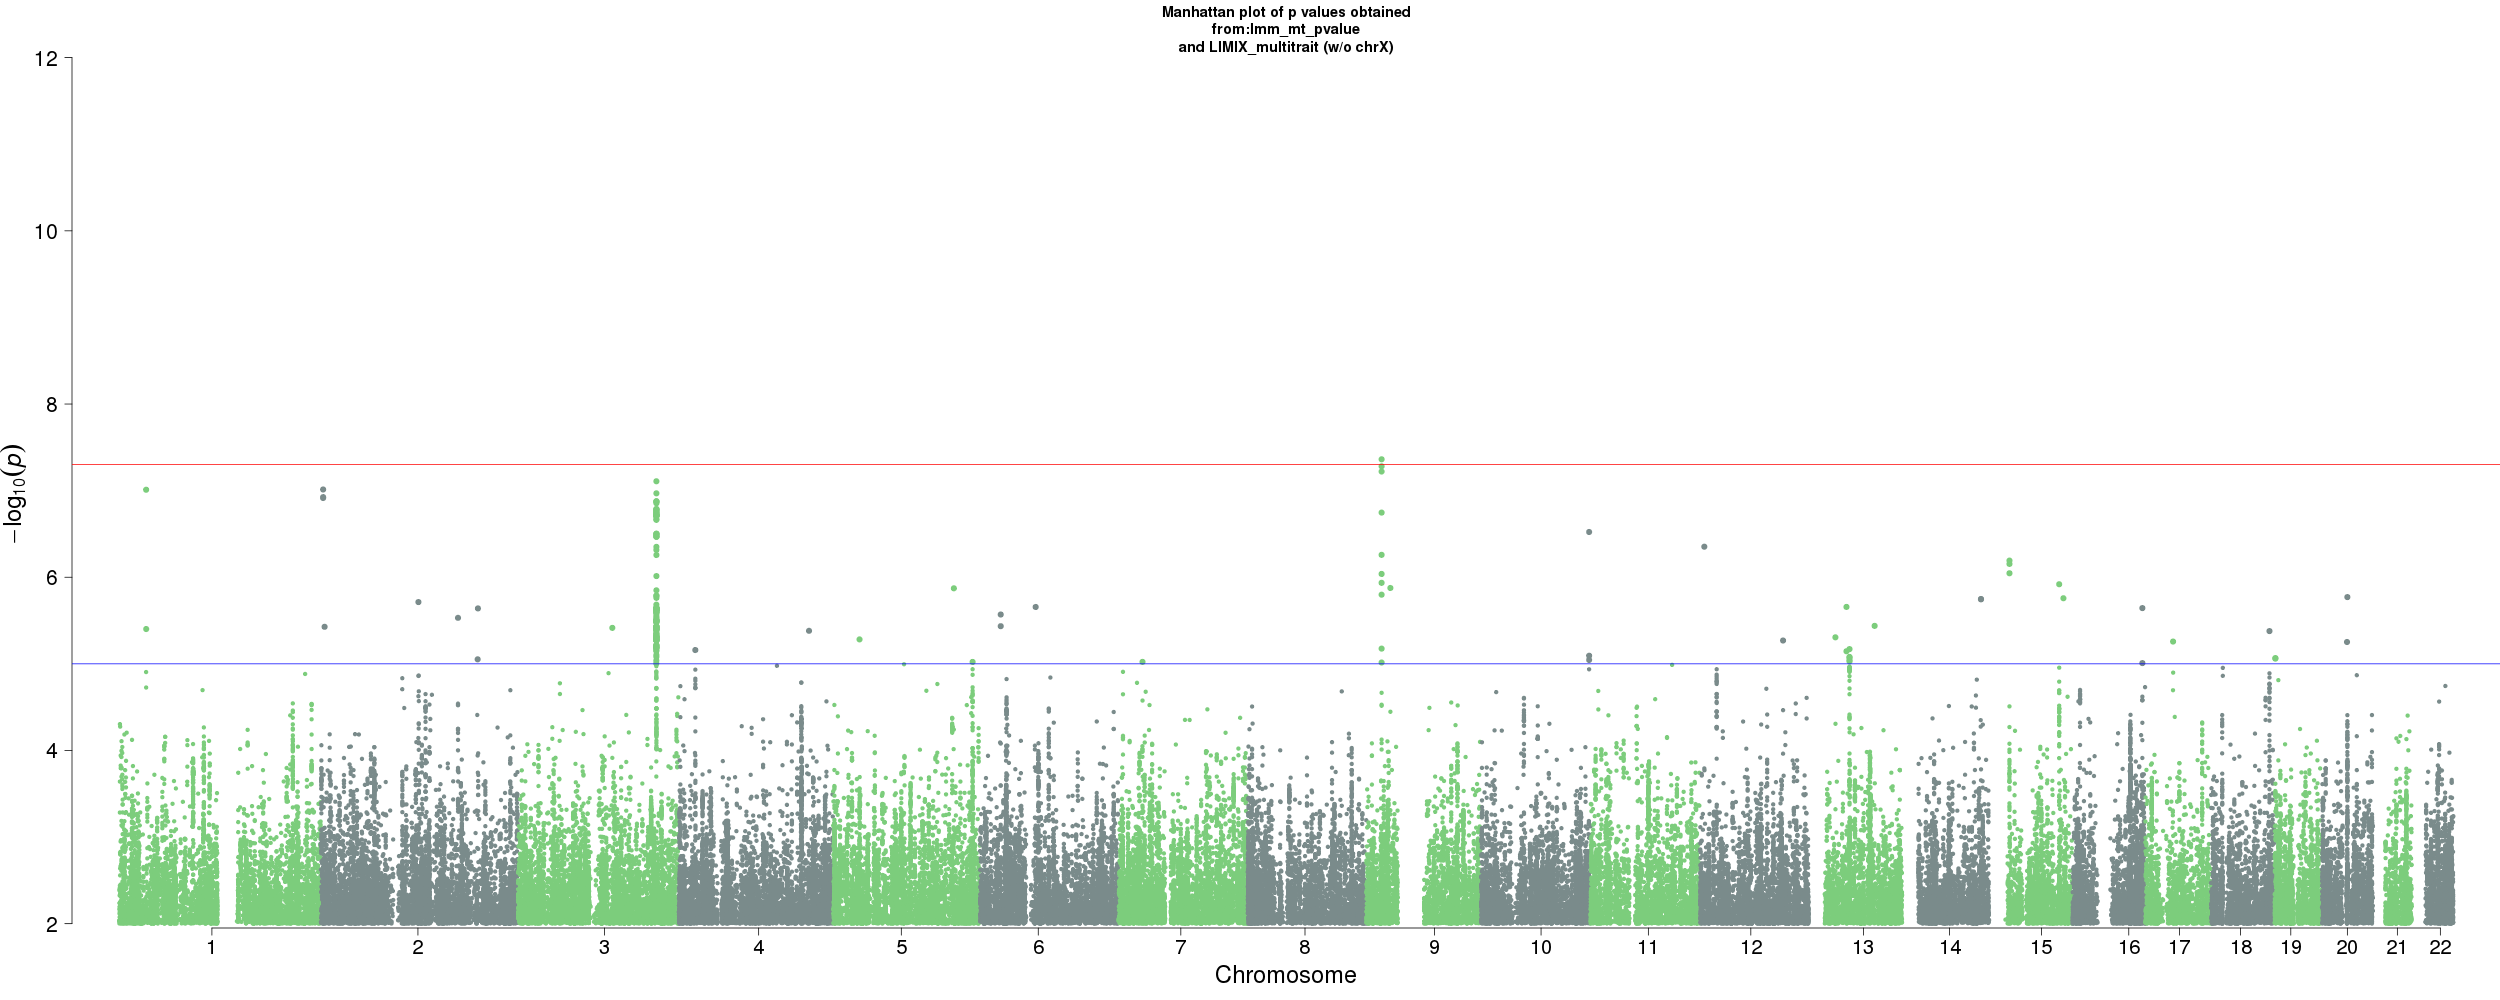
\includegraphics[trim = 0mm 0mm 0mm 100mm, clip, width=1\textwidth]{Figures/lmm_mt_pvalue_LIMIX_multitrait_manhattanplot.png}
	\caption{\textbf{Manhattan plot of genome-wide trabeculation phenotype associations.} Number of CMR slices, maximal apical and basal FD were modeled jointly in an any effect mt-LMM-GWAS with sex, age, height and weight as covariates.}
 	\label{fig:manhattanFD}
\end{figure}

\subsection{Further work}
\begin{itemize}
\item manual QC of genotype cluster plots of SNPs with p-value of less then $5e-4$
\item analysis of ADAMTSL locus for biological function in relation to trabeculation
\item locus zoom of the genomic region
\item potentially improving the presentation of the FD phenotypes to the multi-trait analysis: additional covariates and combinations of the FD measurements
\item replication with UKBiobank data: FD measurements from 2d CMR images scans (access already granted and measurements currently in QC by collaborators)
\end{itemize}
